%%
%% Copyright 2007, 2008, 2009 Elsevier Ltd
%%
%% This file is part of the 'Elsarticle Bundle'.
%% ---------------------------------------------
%%
%% It may be distributed under the conditions of the LaTeX Project Public
%% License, either version 1.2 of this license or (at your option) any
%% later version.  The latest version of this license is in
%%    http://www.latex-project.org/lppl.txt
%% and version 1.2 or later is part of all distributions of LaTeX
%% version 1999/12/01 or later.
%%
%% The list of all files belonging to the 'Elsarticle Bundle' is
%% given in the file `manifest.txt'.
%%

%% Template article for Elsevier's document class `elsarticle'
%% with numbered style bibliographic references
%% SP 2008/03/01
%%
%%
%%
%% $Id: elsarticle-template-num.tex 4 2009-10-24 08:22:58Z rishi $
%%
%%
%%\documentclass[preprint,12pt,3p]{elsarticle}

%% Use the option review to obtain double line spacing
%%\documentclass[preprint,review,12pt]{elsarticle}

%% Use the options 1p,twocolumn; 3p; 3p,twocolumn; 5p; or 5p,twocolumn
%% for a journal layout:
%% \documentclass[final,1p,times]{elsarticle}
%% \documentclass[final,1p,times,twocolumn]{elsarticle}
%% \documentclass[final,3p,times]{elsarticle}
\documentclass[final,3p,times,twocolumn]{elsarticle}
%% \documentclass[final,5p,times]{elsarticle}
%% \documentclass[final,5p,times,twocolumn]{elsarticle}

%% if you use PostScript figures in your article
%% use the graphics package for simple commands
%% \usepackage{graphics}
%% or use the graphicx package for more complicated commands
%% \usepackage{graphicx}
%% or use the epsfig package if you prefer to use the old commands
%% \usepackage{epsfig}


%% The amssymb package provides various useful mathematical symbols
\usepackage{blindtext, graphicx, amsmath, algorithm,algorithmicx, algpseudocode, pifont, algcompatible, comment, layout, amsthm, amssymb, multirow}
\usepackage{enumitem}   
\usepackage{eso-pic}
\usepackage{booktabs}
\usepackage{float, color}
%% The amsthm package provides extended theorem environments
%% \usepackage{amsthm}
\renewcommand{\qedsymbol}{$\blacksquare$}

\usepackage[utf8]{inputenc}
\usepackage[english]{babel}
\usepackage{hyperref} 
\hypersetup{colorlinks=true, linkcolor=black, filecolor=black, urlcolor=cyan, }

\usepackage{caption}
\captionsetup{justification=raggedright, singlelinecheck = false}
\captionsetup[table]{labelformat=simple, labelsep=newline}
\captionsetup[figure]{labelformat=simple, labelsep=period}


%% The lineno packages adds line numbers. Start line numbering with
%% \begin{linenumbers}, end it with \end{linenumbers}. Or switch it on
%% for the whole article with \linenumbers after \end{frontmatter}.
%% \usepackage{lineno}

%% natbib.sty is loaded by default. However, natbib options can be
%% provided with \biboptions{...} command. Following options are
%% valid:

%%   round  -  round parentheses are used (default)
%%   square -  square brackets are used   [option]
%%   curly  -  curly braces are used      {option}
%%   angle  -  angle brackets are used    <option>
%%   semicolon  -  multiple citations separated by semi-colon
%%   colon  - same as semicolon, an earlier confusion
%%   comma  -  separated by comma
%%   numbers-  selects numerical citations
%%   super  -  numerical citations as superscripts
%%   sort   -  sorts multiple citations according to order in ref. list
%%   sort&compress   -  like sort, but also compresses numerical citations
%%   compress - compresses without sorting
%%
%% \biboptions{comma,round}

% \biboptions{}
\newtheorem{theorem}{Theorem}
\newtheorem{lemma}{Lemma}
\newtheorem{definition}{Definition}

\journal{ICT Express}

%\newcommand\AtPagemyUpperRight[1]{\AtPageLowerRight{%
%\put(\LenToUnit{0.8\paperwidth},\LenToUnit{0.9\paperheight}){#1}}}
%\AddToShipoutPictureFG{
%  \AtPagemyUpperRight{{\includegraphics[width=.5cm,keepaspectratio]{logo.png}}}
%}%
%\newcommand\AtPagemyUpperLeft[1]{\AtPageLowerLeft{%
%\put(\LenToUnit{0.85\paperwidth},\LenToUnit{0.9\paperheight}){#1}}}
%\AddToShipoutPictureFG{
%  \AtPagemyUpperLeft{{\includegraphics[width=1.0cm,keepaspectratio]{logo2.jpg}}}
%}%
\begin{document}

\begin{frontmatter}

\title{A Hybrid Approach of ConvLSTM-DT and GPT-4 for Real-time Anomaly Detection Decision Support in Edge-Cloud Environments}
%\author{Author’s Full Name 1\corref{cor1}, Author’s Full Name 2, Author’s Full Name 3}
\author{Radityo Fajar Pamungkas}
\ead{radityofajar@gmail.com}

\author{Ida Bagus Krishna Yoga Utama}
\ead{ibkyutama@ieee.org}

\author{Khairi Hindriyandhito}
\ead{khairihindri@gmail.com}

\author{Yeong Min Jang\corref{cor1}}
\ead{yjang@kookmin.ac.kr}
\address{Department of Electronics Engineering, Kookmin University, Seoul, South Korea}

\cortext[cor1]{Corresponding author}
%\ead{author1@ictexpress.com, author2@ictexpress.com, author2@ictexpress.com}

\begin{abstract}

Anomaly detection is a critical requirement across diverse domains to promptly identify abnormal behavior. Conventional approaches often face limitations with uninterpretable anomaly detection results, impeding efficient decision-making processes. This paper introduces an innovative hybrid approach, the Convolutional Long Short-term Bayesian Neural Network with nonparametric dynamic thresholding (ConvLSTMBNN-DT), for prediction-based anomaly detection. Additionally, the model incorporates fine-tuned GPT-4 to provide human-interpretable explanations in edge-cloud environments.The method achieves outstanding performance with an F1-score and AUC of 0.91 and 0.84, respectively, on collected data, and successfully generates understandable decision support explanations.
\\
2018 The Korean Institute of Communications and Information Sciences. Publishing Services by Elsevier B.V. This is an open access article under the CC BY-NC-ND license (http://creativecommons.org/licenses/by-nc-nd/4.0/).
\end{abstract}

\begin{keyword}
%% keywords here, in the form: keyword \sep keyword
Anomaly detection \sep Large Language Models \sep ConvLSTM-DT \sep Human-understandable explanations \sep Dynamic thresholding
%% MSC codes here, in the form: \MSC code \sep code
%% or \MSC[2008] code \sep code (2000 is the default)
\end{keyword}

\end{frontmatter}

%%
%% Start line numbering here if you want
%%
% \linenumbers

%% main text
\section{Introduction}\label{sec1}
The Internet of Things (IoT) has witnessed exponential growth, reflecting its pervasive impact on various industries. According to recent market reports \textbf{[ref: iot analytics]}, the global IoT market is grew by 18\% in 2022 to 14.3 billion active endpoints. This surge is attributed to the widespread adoption of IoT in diverse sectors, notably smart factories and indoor air quality monitoring. Amidst this growth, the urgency for anomaly detection within IoT systems has become paramount. Anomaly detection plays a pivotal role in mitigating threats by identifying irregularities in data patterns, indicative of potential security breaches. 

Recent studies indicate that the global market size for anomaly detection is predicted to grow with a compound annual growth rate exceeding 16\% \textbf{[ref: marketsearchfuture]}. The benefits of implementing anomaly detection in IoT systems are profound, ranging from preemptive threat mitigation to enhanced system reliability. By identifying and addressing anomalies promptly, businesses can safeguard sensitive data and ensure the uninterrupted functionality of their IoT infrastructure, thereby fostering a secure and resilient technological landscape.

\subsection{Related work}
\begin{figure*}[t]
	\centering
	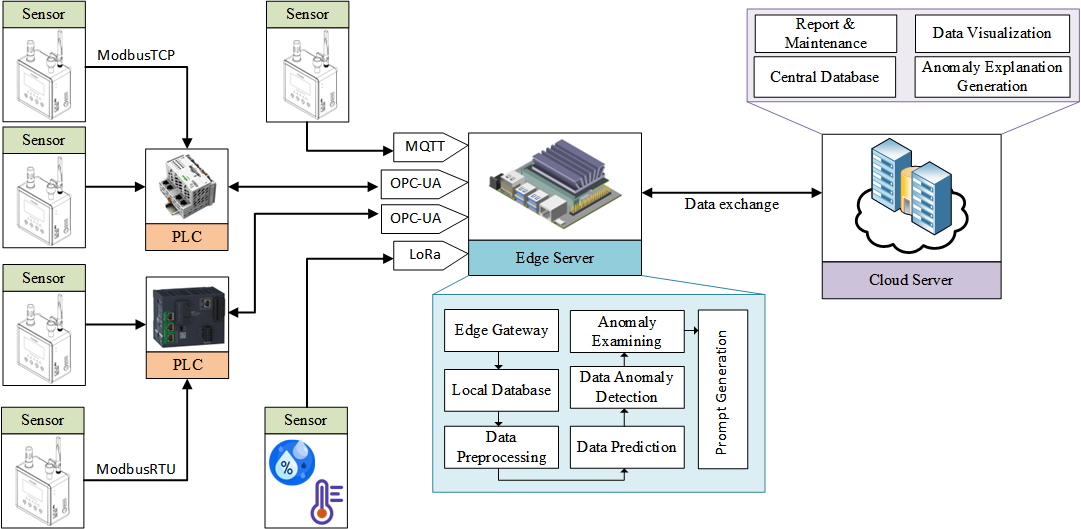
\includegraphics[width=12cm]{Architecture} 
	\caption[width=0.5\paperwidth]{Overall Architecture of Real-time Anomaly Detection Decision Suppoer for Indoor Air Quality Data Monitoring}\label{fig:architecture}
\end{figure*}
Several researchers have proposed different algorithms and methods to detect anomalies lies in time series in streaming scenarios. In recent studies, many researchers tend to use deep learning architecture for anomaly detection in time series due to its powerful data dependency modeling. There are two commonly used deep learning techniques which are prediction-based approaches, and reconstruction-based approaches. \textbf{[Ref: Hundman et al.]} demonstrated the combination of long short-term memory (LSTM) with nonparametric dynamic thresholding for detecting anomalies within telemetry data in rapid changing environment. \textbf{[Ref: Goh et al.]} proposed LSTM as predictor for learning the normal temporal behavior of the data, and subsequently using the Cumulative Sum method to identify anomaly behavior. 
%In \textbf{[Ref: Ergen et al.]}, the authors developed joint architecture that combine LSTM and one-class support vector machines (OC-SVM) that can detect anomalies in time series data without requiring any preprocessing. In \textbf{[Ref: Wu et al.]} presented a method for detecting anomalies in time series with complex seasonality using gated recurrent unit (GRU) for backbone prediction model, then define local trend inconsistency (LTI) that measure the probability of that data’s likelihood of being anomalous.

Reconstruction-based approaches, on the other hand, have also been acknowledged. Unlike prediction-based anomaly detection, these approaches involve recreating the original input through a latent low-dimension representation, ideal for capturing collective anomalies. In \textbf{Ref: Park, Yin, Nguyen, and Wei]}, the authors investigated a hybrid deep learning model that combines LSTM layer in the  shape of autoencoder (AE) architecture to build reconstruction-based unsupervised anomaly detection. 
%In an article \textbf{[Ref: Zhang]}, an adaptive memory network with self-supervised learning (AMSL) based on the convolutional autoencoder structure was proposed to enhance ability in unsupervised anomaly detection and resilience against noise.

While there has been extensive research on time series anomaly detection, the study that incorporates anomaly detection with an explanation for decision support has not been explored to a great extent. In \textbf{[Ref: Gilpin et al.]}, the author’s work represents a pioneering effort that has introduced the emerging field of explanatory anomaly detection, particularly in the realm of system-level explanations through simulated semi-autonomous vehicles. Although previous research is comparable to this paper, the goal of this paper is to design real-time anomaly detection decision support in edge-cloud environments to increase the interpretability and efficiency of tackling anomaly situations. In contrast to previous studies, the anomaly detection algorithm in this article implements a Convolutional LSTM Bayesian neural network with nonparametric dynamic thresholding (ConvLSTMBNN-DT) that accurately forecasts future values and is robust against dynamic environments. Additionally, it employs a fine-tuned generative pre-training version-4 (GPT-4) that can generate human-understandable explanations and enhance interpretability to facilitate quick decision-making.

Therefore, the contributions of our proposed method are summarized as follows:
\begin{itemize}
\itemsep-0.25em 
\item We proposed a novel hybrid approach integrating ConvLSTMBNN-DT and Fine-tuned GPT-4 accurately detects point and contextual anomalies and effectively generates anomaly reasoning and possible solutions for decision support.
\item The conventional schemes are commonly deployed in high power computing capability without considering resource-constraint devices and latency. In contrast, our proposed method deploys the model in edge-cloud environments, considering seamless and real-world edge-computing integrations. Therefore, low-latency anomaly detection on streaming data can be executed.
\item Extensive experiments on generated IAQ datasets demonstrate the effectiveness of the proposed model. Our proposed model outperforms the others anomaly detection models in both F1-score and AUC metrics. Moreover, the proposed method can generate reliable decision support to enhance operation and maintenance system overall performance.
\end{itemize}

The rest of this paper is structured as follows: Section 2 describes the data preprocessing and methodology of the proposed approach. Section 3 presents the experiments settings to demonstrate the efficacy of our proposed method. Section 4 discusses the experiments results. Section 5 brings the conclusion and future work of this manuscript.

\section{Methodology}\label{sec2}

This study proposes anomaly detection on indoor air quality monitoring and providing decision support. In particular, we collect practical air quality data in an indoor setting using our developed IoT platform. The proposed architecture is shown in \textbf{Fig.1}. The edge server collects air quality data such as temperature, humidity, and particulate matter (PM) from several heterogeneous sensors in different rooms. In this study, we mainly focus to perform anomaly detection on three main features in IAQ data which are temperature, humidity, and PM 2.5$\mu m$.

\subsection{Data preprocessing}
It is essential to implement several data processing techniques before training process to improve data quality. Utilizing Pearson's correlation coefficient, we perform feature selection based on a high correlation score.% Subsequently, we set a threshold of $|0.3|$ to eliminate features with lower correlations.
After this feature selection step, we apply the Z-score normalization technique to normalizing the data. This process helps stabilize the gradient descent during training, enabling the model to converge more rapidly.

%\begin{figure}[h]
%	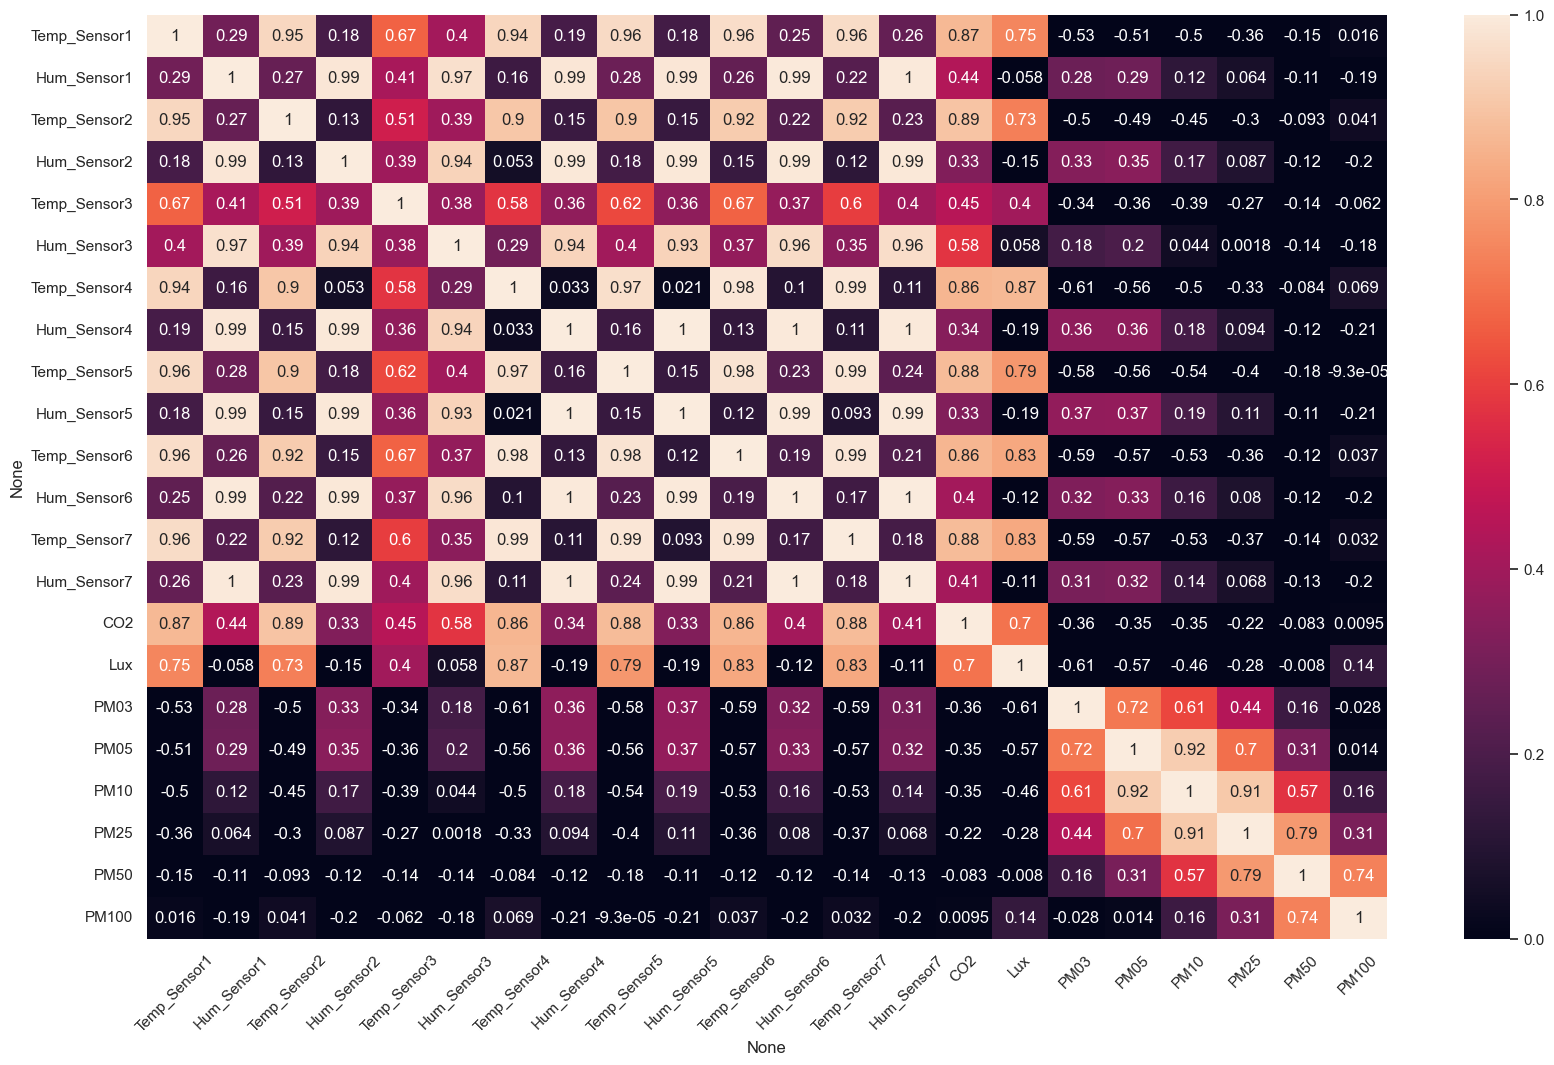
\includegraphics[width=0.5\textwidth]{ConfusionMatrix} 
%	\caption[width=\textwidth]{Correlation Matrix}\label{fig:architecture}
%\end{figure}

\subsection{ConvLSTM-PBNN}
\begin{figure}[h]
	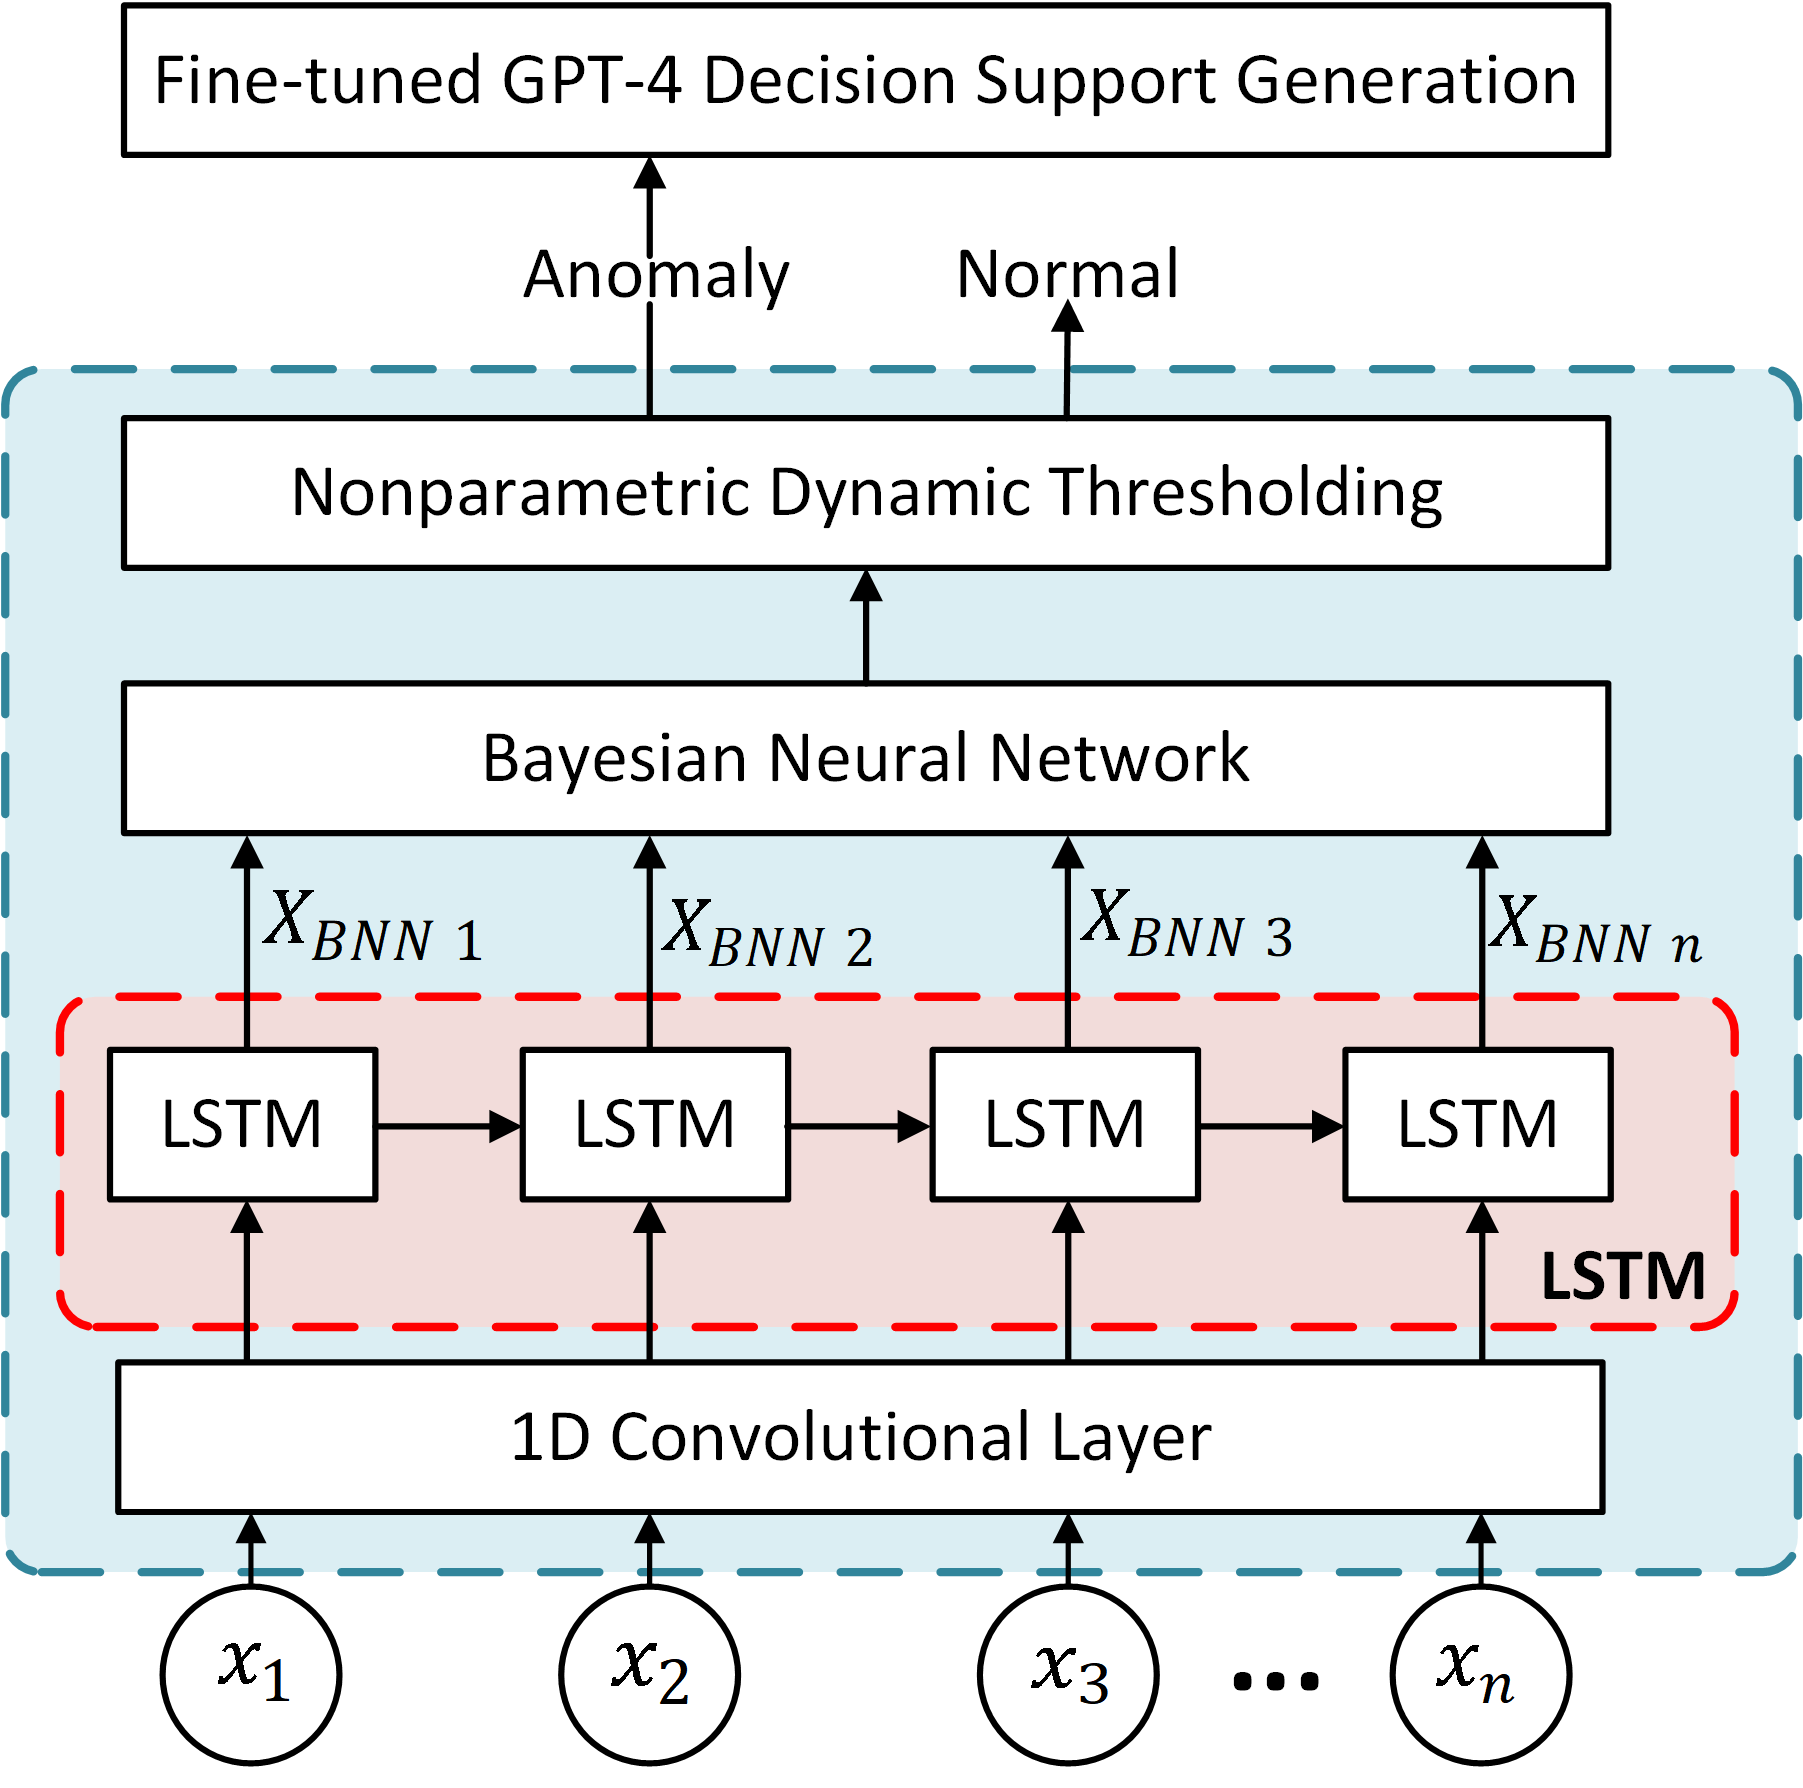
\includegraphics[width=8cm]{ConvLSTMBNNDT} 
	\caption{Architecture of ConvLSTMBNN-DT combine with GPT-4 for Anomaly Detection Decision Support}\label{fig:ConvLSTMBNNDT}
\end{figure}
The prediction model plays an important role in this approach, where accurate forecasting indicates the normal behavior of the system itself. In this method, we modified the LSTM-BNN approach proposed by [Ref: Krishna], which demonstrates remarkable prediction performance compared to common existing models. Fig 3 illustrates the proposed ConvLSTMBNN architecture for the prediction model, followed by passing the output data into thresholding for further analysis and GPT-4 for decision support generation. Modifying the LSTM layer into ConvLSTM, with advantages enhancing the effectiveness of processing both temporal and spatial data, achieves spatio-temporal prediction on multivariate time series data by leveraging a 1D convolutional layer before the LSTM layer. This allows for the incorporation of input from various sensors that may bring spatio-temporal information. The key equations of ConvLSTM are as follows:

\begin{equation}
i(t) = \sigma(W_{xi} \ast X(t) + W_{hi} \ast H(t-1) + W_{ci} \circ C(t-1) + b_i
\label{eq:a}
\end{equation}
\begin{equation}
f(t) = \sigma(W_{xf} \ast X(t) + W_{hf} \ast H(t-1) + W_{cf} \circ C(t-1) + b_f
\label{eq:b}
\end{equation}
\begin{equation}
C(t) = f(t) \circ C(t-1) + i(t) \circ tanh(W-{xc} \ast X(t) + W_{hc} \ast H(t-1) + b_c
\label{eq:c}
\end{equation}
\begin{equation}
o(t) = \sigma(W_{xo} \ast X(t) + W_{ho} \ast H(t-1) + W_{co} \circ C(t) + b_o
\label{eq:d}
\end{equation}
\begin{equation}
H(t) = o(t) \circ tanh(C(t))
\label{eq:e}
\end{equation}

\subsection{Nonparametric Dynamic Thresholding}

After getting the forecast data from the prediction model, thresholding method is needed to determine whether data is classify as normal or abnormal. One main challenge in detecting anomalies in streaming data is the occurrence of data drift, which makes the model and thresholding method irrelevant due to changes in patterns or behavior. To effectively monitor thousands of IoT endpoints influenced by changing environmental conditions, there is a critical need for unsupervised approach to detecting anomalies in dynamic environments. While frequently employed method relies on the assumption of Gaussian distributions for past smoothed errors, enabling swift comparisons with concise representations of previous errors. However, this approach can face challenges when parametric assumptions are violated.

To address this issue, nonparametric dynamic thresholds proposed by \textbf{[Ref: Hundmand et al.]} play a crucial role. This method has been proven to be stable and reliable, minimizing false positives and false negatives against noise and dynamic environments by updating the threshold. Therefore, in this study, we modified and implemented this method in our approach by incorporating continuous learning. \textbf{Algorithm 1} illustrates the step-by-step procedure for prediction-based anomaly detection employing nonparametric dynamic thresholding.

\begin{algorithm}[h]
\caption{Nonparametric Dynamic Thresholding}
\label{DT}

\textbf{Input:} \
$y$ - Streaming data\\
\hspace*{1.1cm} $R$ - Anomaly rate \\
\hspace*{1.1cm} $h$ - Sliding window size \\
\hspace*{1.1cm} $z$ - A factor used to initialize threshold \

\textbf{Output:} 
$A$- a list of indices where anomaly are detected \
$N$- a list of indices of normal data\
\begin{algorithmic}[1]

\WHILE{True}
	\State load the streaming data $y$
	\State $\hat{y} \gets$  Predict the future value of $y$
	\State Calculate deviation $e^{(t)} \gets \hat{y} - y$
	\State Append $e^{(t)}$ into an array $e = [e^{(t-h)}, ... , e^{(t)}]$
	\State Calculate $\mu(e)$ and $\sigma(e)$
	\IF{($T$ is none)}
		\State $T = \mu(e) + z\sigma(e)$
	\ELSE{}
		\State $T= \frac{(\Delta\mu(e)/\mu(e) + \Delta\sigma(e)/\sigma(e))}{(length of A)^2}$
	\ENDIF
	\IF{$e^{(t)} > T$}
		\STATE Append $e^{(t)}$ into $A$ 
	\ELSE{}
		\STATE Append $e^{(t)}$ into $N$
	\ENDIF
	\State Calculate $\Delta\mu(e) = \mu(e) - \mu(N)$
	\State Calculate $\Delta\sigma(e) = \sigma(e) - \sigma(N)$
	\State $r \gets$ length of $e$ $/$ length of $A$
	\IF{$r > R$}
		\STATE Re-train the prediction model
	\ENDIF
	\IF{Length of $e > h$}
		\STATE Remove the oldest data $e^{(t-h)}$ from $e$
	\ENDIF
\ENDWHILE
\end{algorithmic}
\end{algorithm}

\subsection{Fine-tuned GPT-4 integration}
In order to automatically generate understandable decision support based on the provided anomaly detection information, we propose the integration of the (GPT-4 model by OpenAI \textbf{[Ref: GPT]}. While GPT-4 is a powerful and large-scale model, its base version is designed to be general-purpose, which may not fully meet the specific requirements of task-specific anomaly detection decision support, especially when applied to domains like time-series anomaly detection in machine and environmental data. The reasoning generated by the base GPT-4 may be overly general for the intricacies of anomaly detection in these domains.

To address this, fine-tuning GPT-4 with a custom dataset provides several key advantages. It allows for tailoring the model's capabilities to the specific task or domain, leading to higher accuracy and more comprehensive reasoning. Additionally, fine-tuned models can be rapidly deployed for practical applications, making them particularly suitable for tasks where real-time or time-sensitive responses, such as anomaly detection decision support, are essential. In this study, we fine-tuned the GPT-4 model using the OpenAI API \textbf{[Ref: GPT-4 OpenAI API website]} with 50 prompts of anomaly situations and desired responses and trained it for 10 epochs.

\section{Experiments Settings}\label{sec3}
IAQ data covers five days, from October 20th to 25th, 2023, is collected with a one-second sampling frequency. The dataset consists of 7,661,038 data points obtained from seven sensors placed within a single room and split into three set: training, validation, and test set. To simulate anomalies, a total of 300 anomaly data points are manually injected into testing set. This includes 10 point anomalies and 290 contextual anomalies, facilitating comprehensive evaluation of anomaly detection performance.
\subsection{Evaluation metrics}
To assess the performance of the anomaly detection model objectively, we utilize two evaluation metrics to measure its efficiency in detecting anomalies within time series data. In this paper, we consider F1-score and AUC as the metrics for evaluating the model's performance. The formula for each evaluation metric is outlined as follows:
                                                                                                                                                                                            
\begin{equation}\label{eq1}
F1-score = \frac{TP}{TP+1/2(FP+FN)}
\end{equation}

\begin{equation}\label{eq2}
TPR = \frac{TP}{TP+FN}
\end{equation}

\begin{equation}\label{eq3}
FPR = \frac{FP}{FP+TN}
\end{equation}

\begin{equation}\label{eq4}
AUC = \int TPR(FPR) dFPR
\end{equation}

\section{Result and Discussion}\label{sec4}
\begin{figure*}[t]
	\centering
	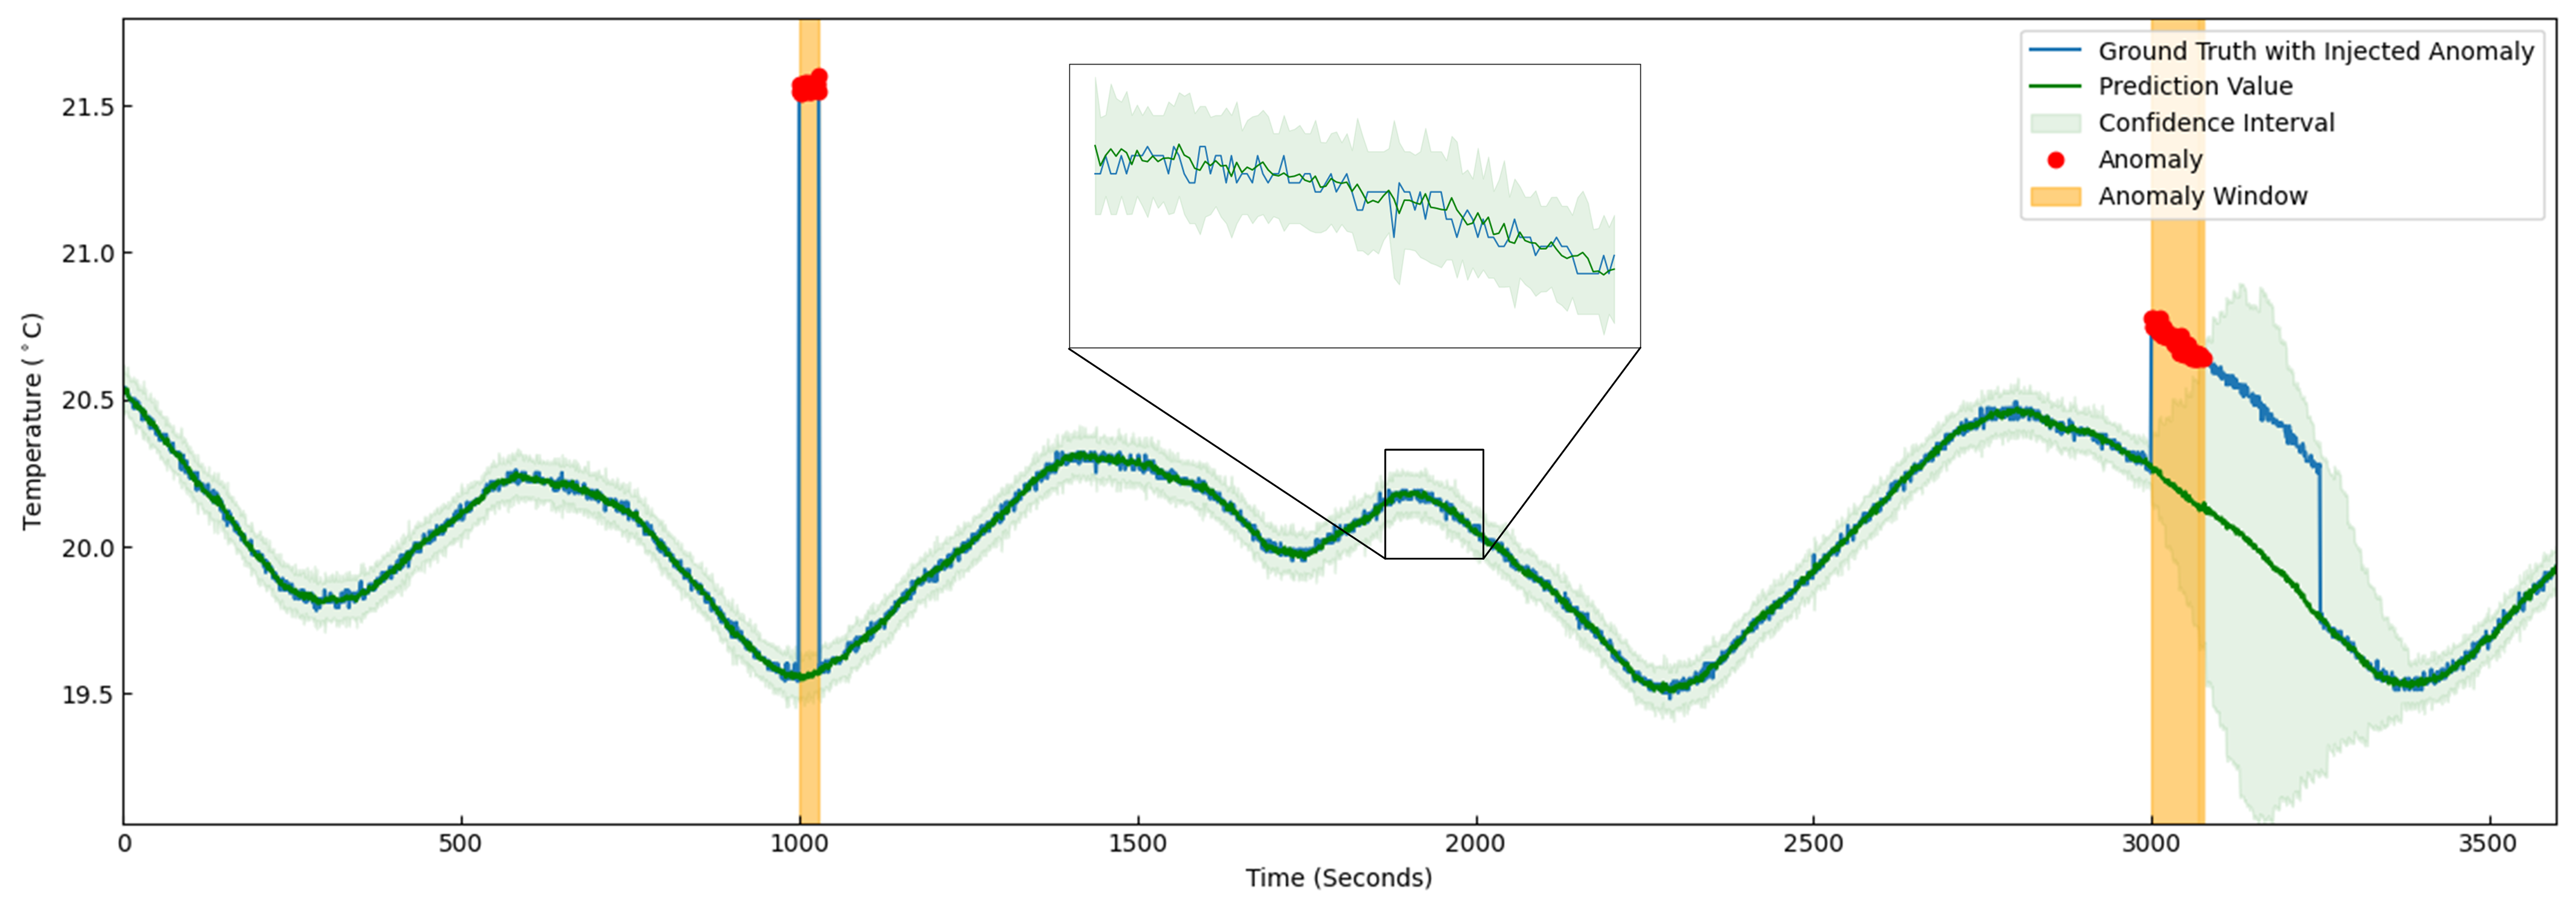
\includegraphics[width=15cm]{Anomaly} 
	\caption[width=0.5\paperwidth]{Anomaly Detection Result using ConvLSTMBNN-DT on Temperature Data}\label{fig:Anomaly}
\end{figure*}

Various anomaly detection models, including the Isolation Forest (IF) from traditional machine learning and deep learning-based approaches such as AE and LSTM-AE, were implemented to evaluate the efficacy of the novel anomaly detection method within a collected dataset with injected point and contextual anomaly data. As depicted in Table 2, presenting the performance analysis outcomes, the proposed model showcases superior performance when compared to other anomaly detection techniques across various features. The evaluation, employing F1-score and AUC metrics, illustrates that the proposed model consistently outperforms its counterparts. This suggests that the proposed model adeptly identifies both generated point anomalies and contextual anomaly data, presenting a noteworthy advancement in comparison to alternative models.

Figure 3 presents the results of the anomaly detection performed by the proposed model. In the plot, the green line represents the ground truth data, the blue line depicts the predicted data, and the green window indicates the confidence interval based on the calculated $T$ value. The zoomed-in plot clearly shows that the proposed model's predictions closely align with the ground truth data, underscoring its robust predictive performance. The model effectively captures the normal pattern or behavior of the data in the 1-hour-ahead prediction window with relatively low error. Notably, the confidence interval dynamically adjusts as the dynamic threshold feature updates. The most significant changes are observed during contextual anomalies, where the confidence interval widens due to an increased number of errors and anomalies in the data. This leads to a lower threshold $T$ value, reflecting the penalization of the total number of anomalies $A$. Therefore, after reach some points, the new-normal incoming data classified as normal.  The results highlight the proposed model's adaptability in dynamic environments, particularly in scenarios where data drift may occur.

The ConvLSTMBNN-DT demonstrates superior anomaly detection performance compared to other models, primarily attributed to the collaborative synergy between ConvLSTM and BNN models, complemented by dynamic thresholding. The ConvLSTMBNN model excels in extracting temporal features from multivariate input data, generating robust predictions by sampling weight values from a learned posterior distribution. This variance in weight values enables the model to dynamically adapt to changing input data. The incorporation of nonparametric dynamic thresholding facilitates automatic adjustments to the threshold, swiftly accommodating data drift and effectively minimizing false positive and false negative detections. The continuous learning aspect further enhances the model's adaptability, ensuring it adeptly captures the temporal patterns within the data. Overall, the ConvLSTMBNN-DT emerges as a powerful anomaly detection solution, proficient in handling dynamic data characteristics and optimizing detection accuracy.

\begin{table}[]
\caption{Performance analysis of anomaly detection models on generated dataset}
\begin{tabular}{lllllll}
\toprule
\multirow{2}{*}{Model} & \multicolumn{2}{c}{Temp} & \multicolumn{2}{c}{Hum}  & \multicolumn{2}{c}{PM} \\ \cline{2-7}
			 &F1                & AUC               & F1              &  AUC            &  F1		&AUC  \\ \hline
IF & 0.86  & 0.81  & 0.82 & 0.77 & 0.88 & 0.82\\
AE      & 0.88 & 0.84 & 0.85 & 0.80 & 0.89  & 0.84\\
LSTM-AE          & 0.87 & 0.82 & 0.86 & 0.81 & 0.90 & 0.86\\ 
Proposed          &\textbf{0.91}& \textbf{0.87} &\textbf{0.90}&\textbf{0.85}&\textbf{0.92}&\textbf{0.87}\\ \hline
\end{tabular}
\end{table}

\begin{figure*}[t]
	\centering
	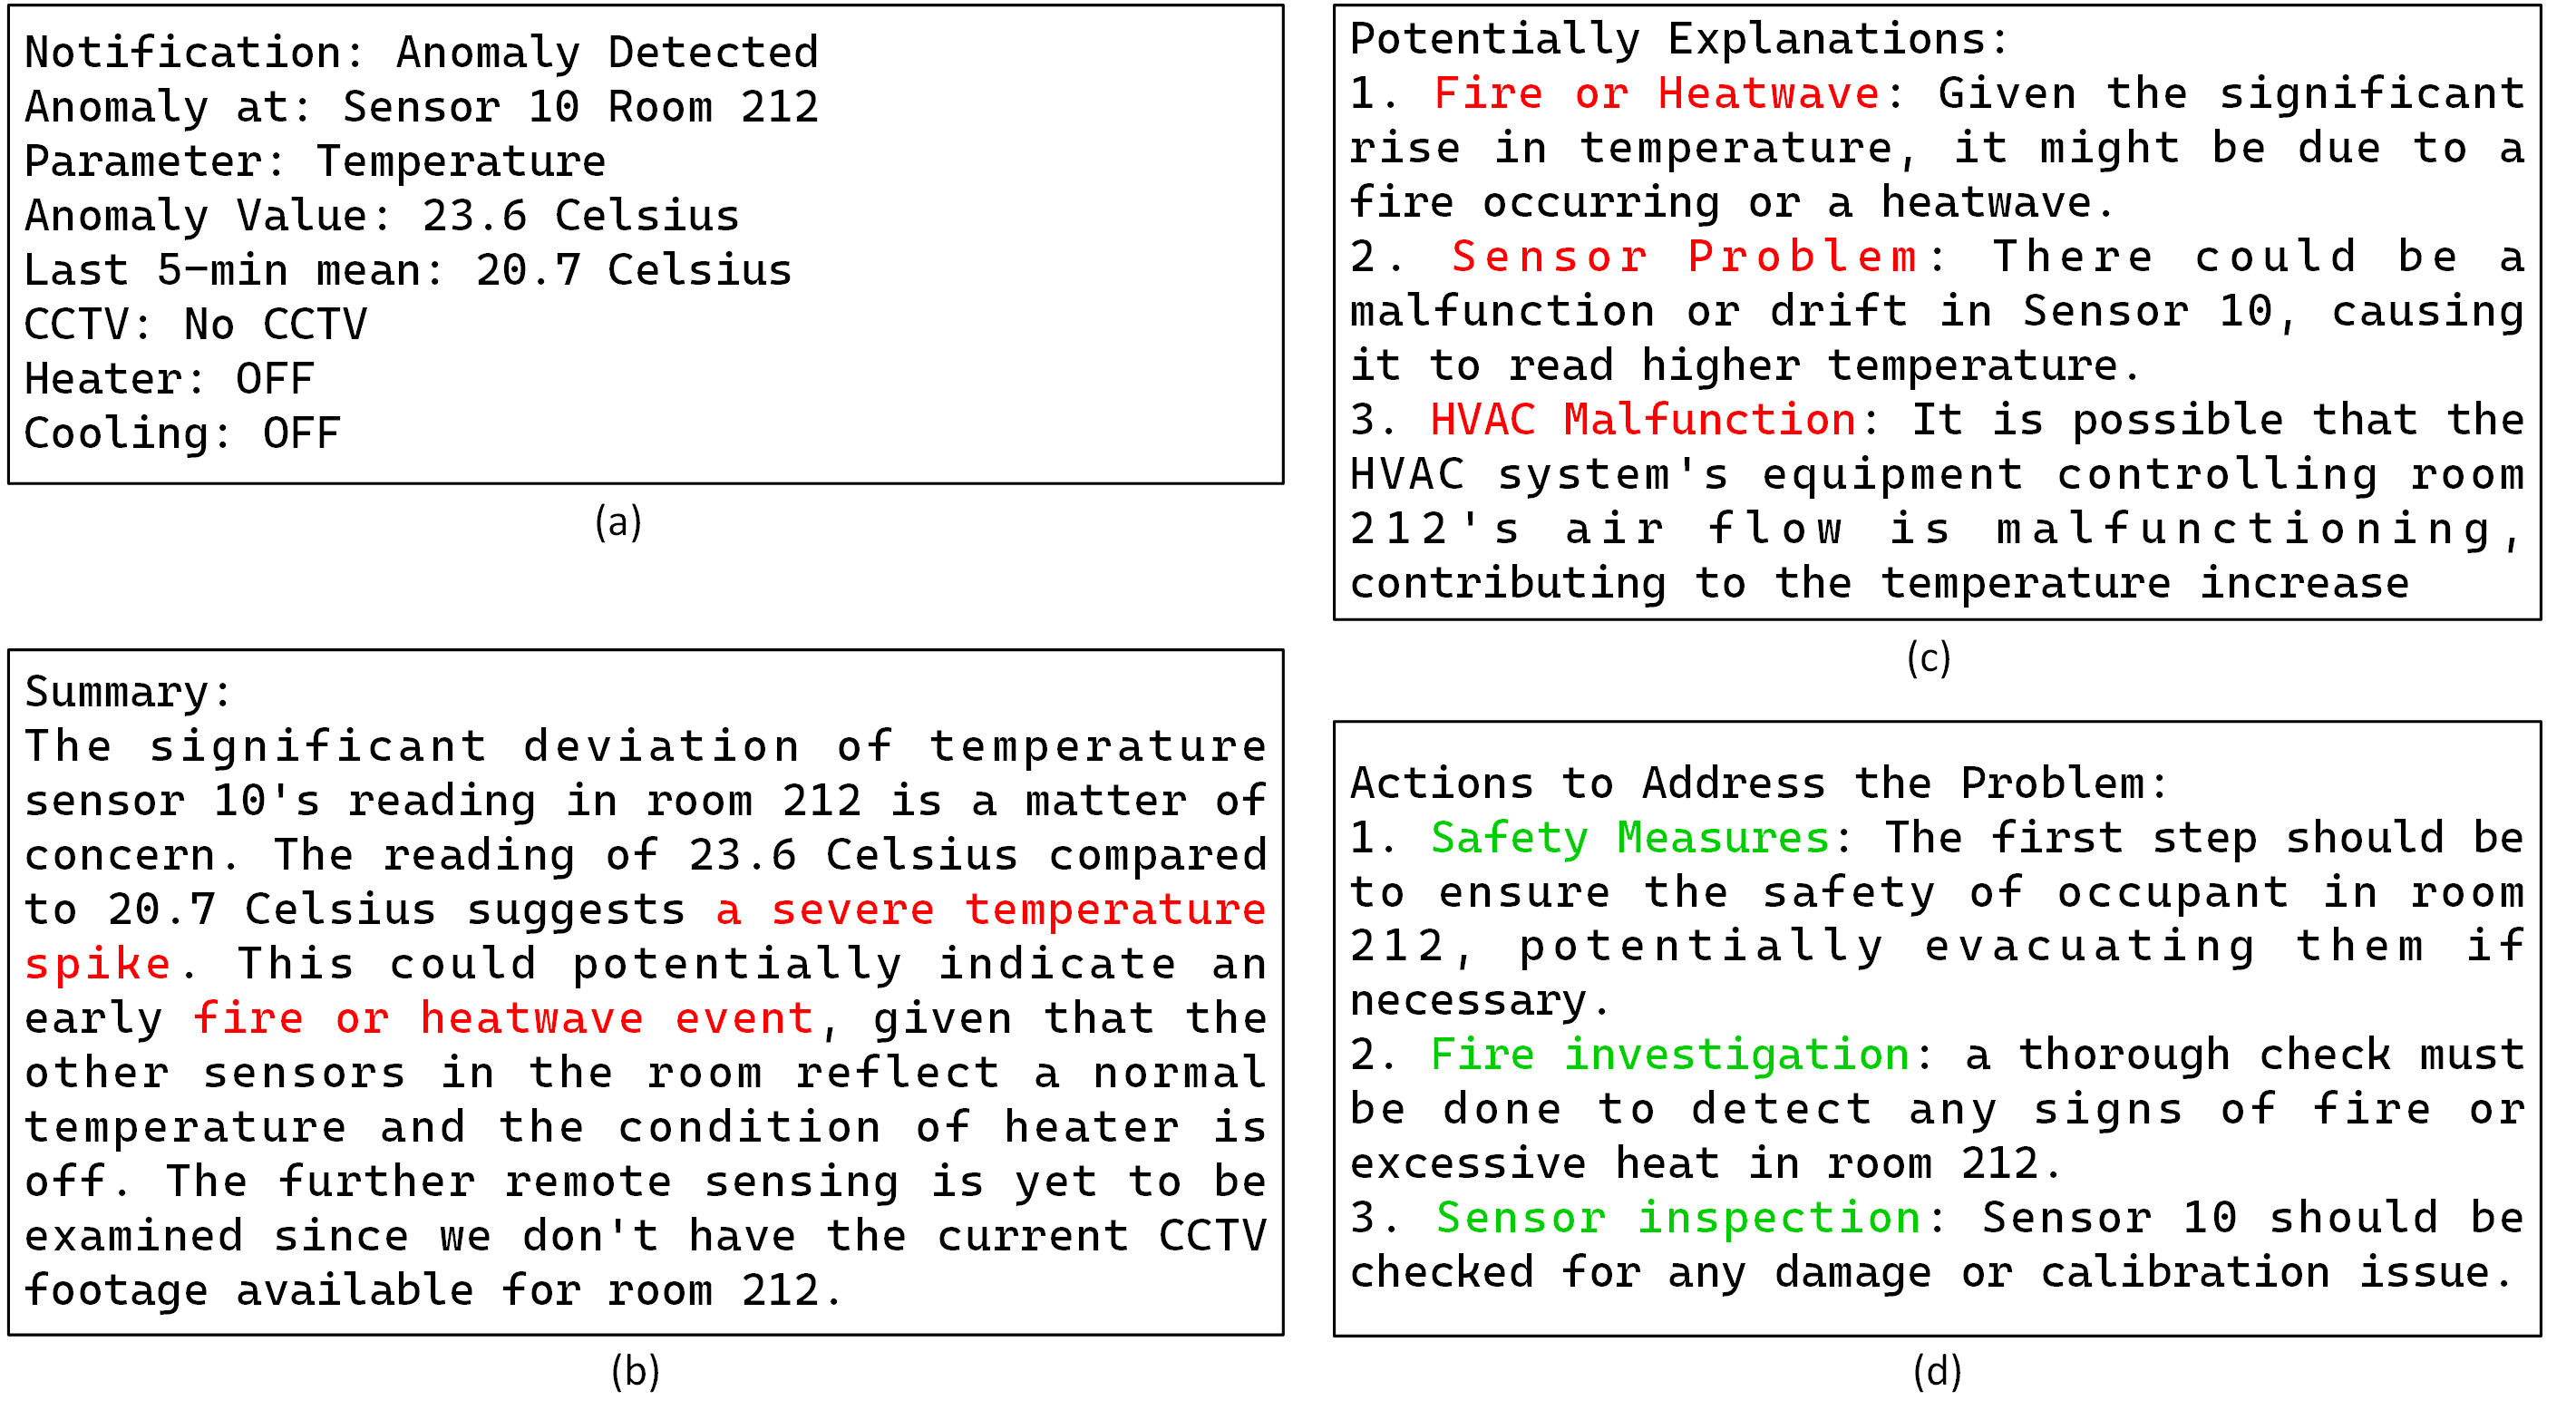
\includegraphics[width=13cm]{NLP} 
	\caption{Result of Decision Support Generated by Fine-tuned GPT-4. (a) Input prompt based on anomaly data, (b) Brief summary of the anomaly data, (c) The potential cause of the anomaly, (d) The possible actions to address the issue}\label{fig:NLP}
\end{figure*}

\section{Conclusion}\label{sec5}
In conclusion, this research introduces a novel hybrid approach that combines prediction-based anomaly detection using ConvLSTMBNN-DT with the fine-tuned GPT-4 model for LLM-based explanation generation, significantly enhancing interpretability and adaptability. By integrating prediction-based algorithms and LLMs, the model not only detects anomalies but also provides human-understandable explanations, making it a powerful tool for quick decision-making in real-world applications. Custom fine-tuning with GPT-4 tailored to the specific anomaly detection task further amplifies interpretability. The presented hybrid approach, along with advanced LLMs, promises to play a pivotal role in improving anomaly detection across various domains.

For future work, enhancing anomaly detection classification could deepen the accuracy of anomaly reasoning. Integrating multimodal sensor fusion, combining time-series data with visual and auditory inputs, may lead to more holistic anomaly detection solutions capable of capturing anomalies across various data modalities. Exploring the integration of reliable control systems for intelligent decision-making in real-time scenarios offers great opportunities.

\section*{Acknowledgments}
This research was supported by the MSIT (Ministry of Science and ICT), Korea, under the ITRC (Information Technology Research Center) support program (IIITP-2023-2018-0-01396) supervised by the IITP (Institute for Information \& Communications Technology Planning \& Evaluation) and Institute of Information \& communications Technology Planning \& Evaluation (IITP) grant funded by the Korea government (MSIT) (No. 2022-0-00590, Industrial small cell system supporting 5G multi-band).

\section*{Declaration of competing interest}
The authors declare that they have no known competing financial interests or personal relationships that could have appeared to influence the work reported in this paper.

\bibliographystyle{elsarticle-num}
% \bibliographystyle{elsarticle-harv}
% \bibliographystyle{elsarticle-num-names}
% \bibliographystyle{model1a-num-names}
% \bibliographystyle{model1b-num-names}
% \bibliographystyle{model1c-num-names}
% \bibliographystyle{model1-num-names}
% \bibliographystyle{model2-names}
% \bibliographystyle{model3a-num-names}
% \bibliographystyle{model3-num-names}
% \bibliographystyle{model4-names}
% \bibliographystyle{model5-names}
% \bibliographystyle{model6-num-names}

\vspace{-0.3cm}

\begin{thebibliography}{1}

\bibitem{els} H. Kwon, K. Kim, C. Lee, The unified UE baseband modem hardware platform architecture for 3GPP specification, J. Commun. Net., 13 (1) (2011) 70-76.

\bibitem{els} T. Roos, P. Myllymaki, H. Tirri, A statistical modeling approach to location estimation, IEEE Trans. Mobile Comput. 1 (1) (2002) 59-69.

\bibitem{els} H. Liu, G. Li, OFDM-Based Broadband Wireless Networks: Design and Optimization. Hoboken, NJ: Wiley-Interscience, 2005.

\bibitem{els} T. L. Marzetta, How much training is required for multiuser MIMO?, in: 2006 Asilomar Conf. Signal. Syst. Comput., Pacific Grove, 2006, pp. 359–363.

\bibitem{els} J. Arrillaga, B. Giessner, Limitation of short-circuit levels by means of HVDC links, in: 1990 IEEE Summer Power Meeting, Los Angeles, 1990, pp. 1-8.

\bibitem{els} J. O. Williams, Narrow-band analyzer, Ph.D. dissertation, Dept. Elect. Eng., Harvard Univ., Cambridge, MA, 1993.

\bibitem{els} J. H. Davis, J. R. Cogdell, Calibration program for the 16-foot antenna, Elect. Eng. Res. Lab., Univ. Texas, Austin, Tech. Memo. NGL-006-69-3, Nov. 15, 1987.

\bibitem{els} RealVNC Ltd. Remote control software [Online]. Available: ftp:// www.realvnc.com


\end{thebibliography}
\end{document}

%%
%% End of file `elsarticle-template-num.tex'.
